
\subsubsection{O que são requisitos}

Em suma, um requisito determina uma capacidade ou condição que deve ser satisfeita pelo sistema. Ou seja, um requisito especifica funções executadas pelo sistema ou uma qualidades que ele deve ter.

Os requisitos podem se relacionar de diversas maneiras, usando as seguintes palavras-chave:  Contém (\textit{containment}), Deriva(\textit{derive}), Satisfaz(\textit{satisfy}), Verifica(\textit{verify}), Rastreia(\textit{trace}) e Copia(\textit{copy}). De maneira geral, existe uma hierarquia entre os requisitos: alguns requisitos juntam-se para formar um requisito central mais importante.

Em SysML, há uma expansão em relação ao UML, em que requisitos podem ter relacionamentos não só entre si, mas também com elementos de design, análises e casos de testes. 


\subsubsection{Estrutura dos diagramas de requisitos}
O diagrama de requisitos representa o que é necessário para o sistema em questão funcionar conforme esperado. Seu objetivo é permitir a visualização da hierarquia e das relações entre os requisitos durante a especificação de um projeto. 

A ideia é organizar os requisitos de alto nível e baixo nível de maneira a deixar clara sua diferenciação, mas mantendo suas ligações. 

 Relações de contenção são representado por uma ligação sólida com uma cruz dentro de uma circunferência (\textit{crosshair}), as outras são relações seguem a conexão de associação detalhada em 2.2.1.

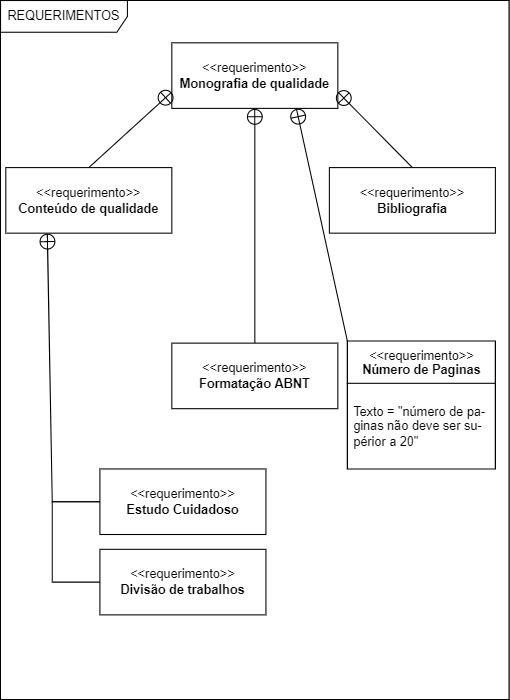
\includegraphics[width=\textwidth/2,height=\textheight,keepaspectratio]{figures/diagrama de requistos exemplo 1.png}
% \begin{figure}[h]
% \centering
% 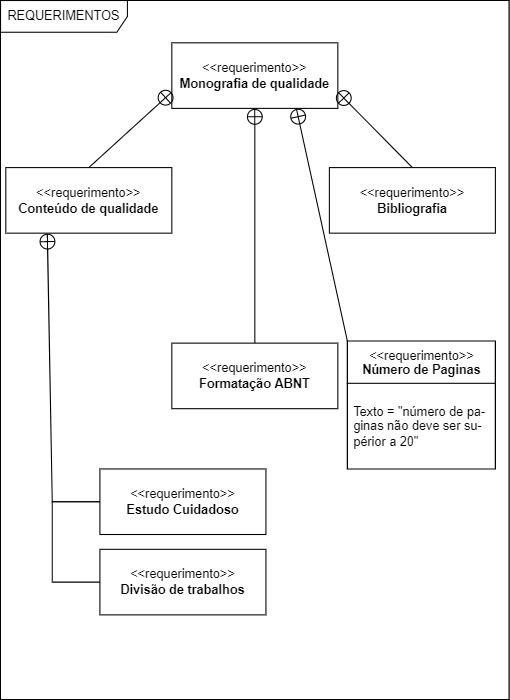
\includegraphics[width=0.75\textwidth]{figures/diagrama de requistos exemplo 1.png}
% \caption{Diagrama de Requisitos}
% \label{fig:package_diagram}
% \end{figure}
